\section{Implementacja}
W tym rozdziale przedstawiona zostanie implementacja w postaci modułowej. Na początek jednak, warto wyróżnić dostępne biblioteki oraz te użyte w realizacji projektu. Każda operacja wchodząca w skład algorytmu rozpoznawania koloru samochodów osobowych zostanie przybliżona. Oprócz znaczenia i krótkiego opisu każdego z modułów, przekazana zostanie również jego programowa implementacja w postaci krótkiego listingu kodu źródłowego.

\subsection{Dostępne i użyte technologie}

Do wykonania projektu użyty został język programowania \textbf{Python}. Ten wybór uzasadniony jest przez:
\begin{enumerate}
    \item Osobiste obycie oraz doświadczenie z językiem 
    \item Ogromną dostępność bibliotek oraz rozwiązań pozwalających na implementację:
        \begin{itemize}
            \item Przetwarzania obrazu (OpenCV, numpy, scikit-image, pillow)
            \item Uczenia maszynowego (scikit-learn, tensorflow, keras)
            \item Ogólnej wygody i wydajności przy pracy ze zbiorami danymi (numpy, pandas)
            \item Wykrywania obiektów z obrazu (OpenCV, OpenCV + YOLOv3 \cite{yolov3})
        \end{itemize}
    \item Każde z używanych narzędzi cieszy się rozbudowaną, nieustannie utrzymywaną dokumentacją oraz wsparciem.
\end{enumerate}

Kolejne technologie wraz z ich implementacjami przytaczane będą zgodnie z kolejnością ich użycia w algorytmie.

\subsection{Wczytanie zbioru danych}
Wczytujemy do pamięci operacyjnej obrazy ze zbioru danych za pomocą bibliotek \textbf{OpenCV} oraz \textbf{os}.
Wbudowana biblioteka języka python - \textbf{os}, pozwala na operacje na plikach oraz folderach (także listowanie ich zawartości).

\begin{lstlisting}[language=Python, caption=Wczytanie zbioru danych]
import os
import cv2 as cv

data_path = r'assets/train' # Glowny folder danych
data = { "images": [], "label": [] }

for subdir in os.listdir(data_path): # Przejscie przez kazdy podfolder
    current_path = os.path.join(data_path, subdir)

    for file_name in os.listdir(current_path): # Przejscie przez kazdy plik w podfolderze
        image_path = os.path.join(current_path, file_name)
        image = cv.imread(image_path)
        data["imagees"].append(image)
        data["label"].append(subdir)
\end{lstlisting}

W zmiennej \textbf{data} (typu słownik) agregowane są etykiety danych - \textbf{label} - oraz dane liczbowe wczytanych obrazów - \textbf{images} (każdy obraz to tablica wartości kanałów RGB każdego piksela). Program zakłada strukturę plików, w której w folderze \textbf{assets/train} znajdują się podfoldery, których nazwy to etykiety zawartych w nich obrazów.

\subsection{Wykrywanie obiektów}
Do detekcji pojazdów użyta została biblioteka \textbf{OpenCV} w połączeniu z publicznie dostępnym, wytrenowanym modelem \textbf{YOLOv3}. Model ten został wytrenowany na podstawie zbioru danych "\null{}Pospolitych Obiektów w Kontekście" (COCO, z ang. Common objects in context) \cite{coco}. Oprócz samochodów, owy zbiór danych zawiera w sobie 79 innych klas obiektów.

Działanie obu bibliotek jest komplementarne w procesie detekcji. Za pomocą OpenCV tworzymy głęboką sieć neuronową, której nadajemy wagi dostępne w wyuczonym modelu YOLOv3. Przepuszczamy obrazy przez głęboką sieć, odnajdując wszystkie instancje pożądanej klasy. W wyniku otrzymujemy współrzędne każdej odnalezionej instancji w obrazie w formacie wymiarów prostokąta opisanego na instancji (wysokość, szerokość oraz współrzędne lewego, górnego rogu prostokąta względem lewego górnego rogu oryginalnego obrazu).\\

\begin{lstlisting}[language=Python, caption=Przetworzenie obrazu za pomocą głębokiej sieci neuronowej]
import cv2 as cv
# Inicjalizacja glebokiej sieci neuronowej
deep_neural_network = cv.dnn.readNetFromDarknet(
                    r"config/yolov3-320.cfg", 
                    r"config/yolov3.weights")
# Funkcja przetwarzajaca obraz za pomoca sieci            
def dnn_passthrough(image):
    blob = cv.dnn.blobFromImage(
            image, 1 / 255, # dane liczbowe obrazu oraz zadane skalowanie
            (width_height, width_height), # rozmiary powstalego blobu
            [0, 0, 0], 1, crop=False) # konwersja z formatu BGR do RGB
    deep_neural_network.setInput(blob)
    layers_names = deep_neural_network.getLayerNames()
    output_names = [(layers_names[i - 1]) 
                for i in deep_neural_network.getUnconnectedOutLayers()]
    return deep_neural_network.forward(output_names)
\end{lstlisting}

Tworzymy model głębokiej sieci neuronowej za pomocą metody biblioteki OpenCV \textbf{readNetFromDarknet}, której jako parametry podajemy pliki konfiguracyjne modelu YOLOv3. 

Funkcja \textbf{dnn\_passthrough} służy do przetworzenia obrazu przez ową sieć. Najpierw obraz konwertujemy do formatu \textbf{blob}. W tym przypadku oznacza to jedynie skalowanie obrazu o współczynnik 1/255 (zmniejszenie) oraz zamiana kolejności kanałów kolorów z formatu BGR do RGB (funkcję biblioteki OpenCV standardowo operują na danych liczbowych obrazu w układzie BGR). Przejście do formatu blob jest wykonywane, ponieważ sieci neuronowe dostępne w OpenCV były optymalizowane pod kątem właśnie tego formatu. Następnie mówimy metodzie \textbf{forward}, wartości których warstw sieci nas interesują podając ich nazwy jako parametr. Oczywiście interesują nas jedynie warstwy wyjściowe (wynik sieci neuronowej) - podajemy więc zmienną \textbf{output\_names}, zawierającą nazwy warstw wyjściowych.

\begin{lstlisting}[language=Python, caption=Znalezienie wymiarów prostokątów opisanych na wykrytych siecią obiektach]
import cv as cv2, numpy as np

def find_objects(dnn_outputs, image):
    height, width, _ = image.shape # Rozmiary obrazu wejsciowego
    bounding_boxes, class_indexes, confidences = [], [], []

    for output in dnn_outputs:
        for determinant in output:
            scores = determinant[5:]
            class_index = np.argmax(scores)
            confidence = scores[class_index]

            if confidence > confidence_threshold and class_names[class_index] == 'car':
                w = int(determinant[2] * width)
                h = int(determinant[3] * height)
                x = int((determinant[0] * width) - w / 2)
                y = int((determinant[1] * height) - h / 2)
                bounding_boxes.append([x, y, w, h])
                class_indexes.append(class_index)
                confidences.append(float(confidence))

    indices = cv.dnn.NMSBoxes(
        bounding_boxes,
        confidences,
        confidence_threshold,
        non_maximum_suppresion_threshold)

    return [bounding_boxes[i] for i in indices]
\end{lstlisting}

\pagebreak

Funkcja \textbf{find\_objects} przechodzi przez listę wszystkich wyników detekcji głębokiej sieci. Jeśli wykryty został samochód oraz pewność detekcji jest wyższa niż zadany przez nas próg, wyliczane zostają współrzędne lewego górnego rogu prostokąta opisanego na wykrytym obiekcie względem lewego górnego rogu oryginalnego obrazu oraz szerokość i wysokość tego prostokąta. Współrzędne prostokąta, wraz z pewnościami ich detekcji oraz klasą, która została wykryta (dla nas to zawsze samochód) są przetrzymane w zmiennych. 

Na podstawie współrzędnych prostokąta, pewności i klasy detekcji oraz dodatkowo zadanego progu spłaszczania prostokątów, metoda \textbf{NMSBoxes} redukuje nachodzące na siebie, redundantne prostokąty. Dzięki tej operacji, wynik wyjściowy działania funkcji find\_objects to pojedynczy prostokąt dla każdego wykrytego obiektu.

\begin{lstlisting}[language=Python, caption=Użycie zaimplementowanej detekcji i jej wizualizacja]
import cv2 as cv

image_path = r'assets/0197.jpg'
image = cv.imread(image_path)
outputs = dnn_passthrough(image)

try:
    boxes = findObjects(outputs, image)
except:
    print("Couldn't find a car in given frame")
    
for box in boxes:
    x, y, w, h = box[0], box[1], box[2], box[3]
    cv.rectangle(image, (x, y), (x + w, y + h), (0, 255, 0), 2)
cv.imshow('Showcase', image) # Wyswietlenie obrazu wynikowego
cv.waitKey(0) # Prewencja przedwczesnego zamkniecia sie okna z wizualizacja
\end{lstlisting}

Dzięki zamknięciu części operacji w osobnych funkcjach, przykładowe użycie detekcji jest relatywnie proste. Po wczytaniu obrazu, przepuszczamy go przez głęboką sieć neuronową za pomocą funkcji \textbf{dnn\_passthrough}. Potem z wyniku tej operacji wyciągamy współrzędne pojedynczych prostokątów opisanych na wykrytych obiektach dzięki użyciu funkcji \textbf{find\_objects}. Na koniec, na podstawie współrzędnych możemy umieścić na oryginalnym obrazie prostokąty oraz go wyświetlić, w ten sposób wizualizując działanie detekcji. Wynik działania zaimplementowanej detekcji:

\begin{figure}[h!]
    \begin{center}
        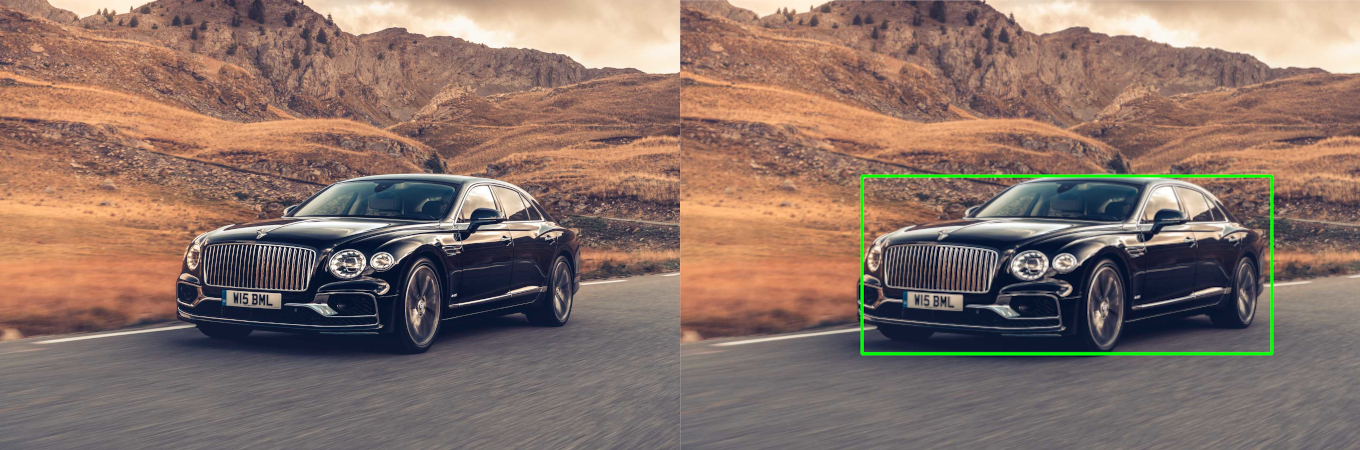
\includegraphics[scale=1.43]{img/detection_visualization.jpg}
    \end{center}
    \caption{Obraz przed i po detekcji samochodu\protect\footnotemark}
    \label{fig:cnn_arch_pic}
\end{figure}

\footnotetext{Użyte zdjęcie samochodu dostępne pod adresem:      \url{https://images.hgmsites.net/hug/2020-bentley-flying-spur_100720091_h.jpg}}

\subsection{Wycięcie obiektów oraz wyodrębnienie cech znaczących}
Po operacji detekcji, wycinamy wszystkie instancje odnalezionych samochodów z obrazu na podstawie otrzymanych w trakcie detekcji współrzędnych. W tym celu posługujemy się biblioteką numpy. Dokonane jest to, przez proste zapisanie do osobnej tablicy obrazu okrojonego (z ang. array slicing) o współrzędne otrzymane w trakcie detekcji.

\begin{lstlisting}[language=Python, caption=Wycięcie obiektów]
image_cropped = image[y: y + h, x: x + w]
\end{lstlisting}
\begin{math}
x
\end{math}
- odległość górnego, lewego wierzchołka prostokąta opisanego na wykrytym obiekcie od lewej granicy obrazu oryginalnego\\
\begin{math}
y
\end{math}
- odległość górnego, lewego wierzchołka prostokąta opisanego na wykrytym obiekcie od górnej granicy obrazu oryginalnego\\
\begin{math}
w
\end{math}
- szerokość prostokąta opisanego na wykrytym obiekcie\\
\begin{math}
h
\end{math}
- wysokość prostokąta opisanego na wykrytym obiekcie\\

Biblioteka OpenCV zawiera metodę \textbf{calcHist} służącą do ekstrakcji histogramu kolorów z danych liczbowych obrazu. Otrzymujemy w ten sposób informację o nasyceniu kanałów R, G oraz B w obrazie, bez ich lokalizacji w obrazie. To znacznie zmniejsza wielkość wynikowej tablicy liczbowej, a więc poprawia wydajność trenowania i działania perceptronu wielowarstwowego.

\begin{lstlisting}[language=Python, caption=Wyodrębnienie cech znaczących]
 features = []

hist = cv2.calcHist(
    [image_cropped], # Dane liczbowe obiektu wycietego z obrazu
    [0, 1, 2], # Ilosc kanalow (3 kanaly - RGB)
    None, # Maska
    (16, 16, 16),  # Rozdzielczosc dla kazdego z kanalow
    [0, 256, 0, 256, 0, 256]) # Zakres kolorow ktore chcemy wziac pod uwage dla kazdego z kanalow
hist = cv2.normalize(hist, hist).flatten() # Normalizacja histogramu

features.extend(hist)
\end{lstlisting}

Zmienna \textbf{features} (typu listy) przechowuje dane liczbowe histogramu kolorów otrzymanego w trakcie operacji wyodbrębniania cech znaczących.

\subsection{Stworzenie modelu uczenia maszynowego}

Biblioteka \textbf{scikit-learn} pozwala na implementację dowolnej konfiguracji uczenia maszynowego w prosty i przejrzysty sposób. Użyta konfiguracja modelu została uzyskana eksperymentalnie. Proces szukania owych parametrów został opisany w następnej sekcji (\ref{sec:grid}). Dzięki użyciu zaszytych w bibliotece scikit-learn metod oraz klas, można w następujący sposób zdefiniować model perceptronu wielowarstwowego:

\begin{lstlisting}[language=Python, caption=Definiowanie modelu MLP]
from sklearn.neural_network import MLPClassifier
mlp = MLPClassifier(
        hidden_layer_sizes=(100, 50, 25), # 1
        max_iter=5000, # 2
        solver="adam", # 3
        activation="relu", # 4
        learning_rate="adaptive", # 5)
\end{lstlisting}

\null{}

Zdefiniowany w ten sposób model MLP cechuje się:
\begin{enumerate}
    \item Trzema warstwami ukrytymi, o liczebnościach kolejno 100, 50 i 25 sztucznych neuronów
    \item Maksymalną ilością 5 tysięcy powtórzeń modyfikacji wag na podstawie funkcji kosztu (MSE).
    \item Funkcją optymalizacji wag w postaci algorytmu działającego na podstawie gradientu stochastycznego (z ang. stochastic gradient)
    \item Funkcją aktywacji Rectified Linear Unit (ReLU)
    \item Zmiennym współczynnikiem uczenia. Wagi są z każdą iteracją dopasowywane z zmienną czułością, pozwalając na ich dokładniejsze dostrojenie.
\end{enumerate}

\subsection{Dobór parametrów modelu MLP}
\label{sec:grid}

Użyte w definiowaniu modelu parametry nie są oczywiście przypadkowe. W celu znalezienia parametrów najbliższych optymalnym (w przystępnym czasie) możemy posłużyć się klasą \textbf{GridSearchCV} dostępną w module \textbf{scikit-learn}. 

W swojej istocie, klasa ta działa następująco: po podaniu jej przestrzeni parametrów, konstruuje z wielu wariacji zadanych parametrów nowe modele, trenuje je, a następnie generuje dla nich metryki jakościowe. 

Po okresie tworzenia, trenowania i walidacji jakości modeli, w zmiennej \textbf{best\_params\_} przechowywane są parametry modelu, który wykazał się najwyższymi wynikami.

\begin{lstlisting}[language=Python, caption=Przykład użycia klasy GridSearchCV]
from sklearn.model_selection import GridSearchCV
parameter_space = {
    'hidden_layer_sizes': [(100, 50, 25), (100, 70, 40, 10),
                (100, 45, 10), (70, 35, 17), (70, 52, 35, 17)],
    'max_iter': [5000],
    'activation': ['tanh', 'relu'],
    'solver': ['sgd', 'adam'],
    'alpha': [0.0001, 0.05, 1e-3],
    'learning_rate': ['constant','adaptive'],
}
best_mlp = GridSearchCV(MLPClassifier(), parameter_space,  
            n_jobs=-1, # Ilosc uzywanych procesorow logicznych (-1 oznacza uzycie wszystkich dostepnych w systemie)
            verbose=4) # logowanie duzej ilosci komunikatow
best_mlp.fit(X_train, y_train) # trenowanie i walidacja nowych modeli

print(mlp_from_grid.best_params_)
\end{lstlisting}

Parametry zawierane w przestrzeni są wybierane bez konkretnej reguły, a raczej na podstawie doświadczenia i intuicji. Trudno przewidzieć jak połączenia poszczególnych wartości mogą ze sobą współgrać w skomplikowanych przypadkach, dlatego potrzebujemy programowej metody, która uzasadnia wybrane przez nas parametry modelu.\\

Warto wspomnieć, iż konstruktor klasy GridSearchCV pozwala na konfigurację związaną z współbieżnością procesu trenowania modeli. Możemy podać ilość procesorów logicznych, które mają być przeznaczone na rzecz wykonania trenowań lub pozwolić tej klasie na programowe wykrycie ilości dostępnych procesorów logicznych w naszym systemie i utworzenie właśnie tylu procesów.
    
\pagebreak
    
\subsection{Trenowanie modelu i przewidywanie}
Korzystając z wcześniej zdefiniowanego obiektu modelu perceptronu wielowarstwowego możemy wytrenować model na podstawie przetworzonych danych (po detekcji, wycięciu oraz ekstrakcji histogramu kolorów). Do tego użyjemy metody \textbf{fit}, której podajemy jako argumenty wspomniane dane oraz ich etykiety.

Po wytrenowaniu modelu, możemy za jego pomocą zacząć generalizować kolory aut nowych instancjach obrazów samochodów. Wtedy jako argument metody \textbf{predict} podajemy przetworzone dane nowego obrazu. Metoda zwróci nam wówczas wykryty kolor samochodu.

\begin{lstlisting}[language=Python, caption=Trenowanie modelu i przewidywanie]
mlp.fit(X_train, y_train)

y_pred = mlp.predict(X_test)
\end{lstlisting}
\begin{math}
X\_train
\end{math}
- dane trenujące\\
\begin{math}
X\_test
\end{math}
- dane testowe\\
\begin{math}
y\_train
\end{math}
- etykiety danych trenujących\\
\begin{math}
y\_pred
\end{math}
- przewidziany wynik na podstawie danych testowych\\


% \begin{figure}[h!]
%     \begin{center}
%         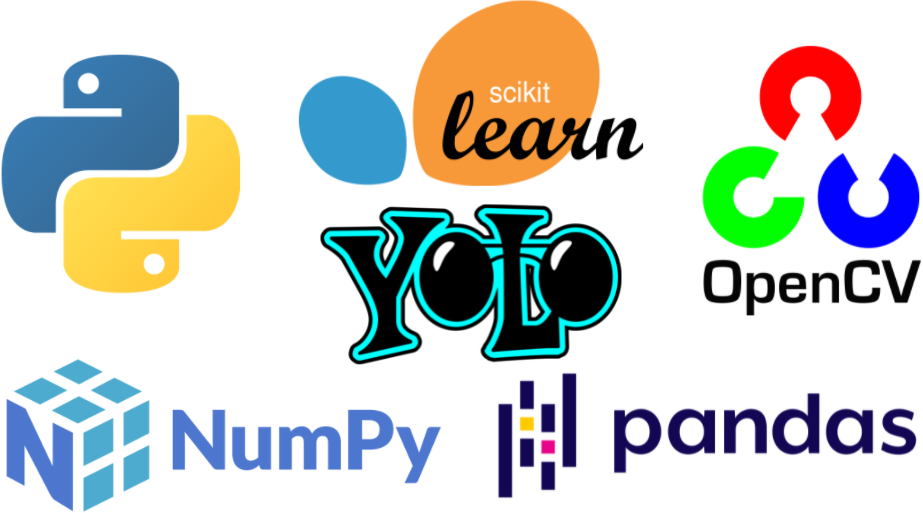
\includegraphics[scale=0.5]{img/technologie.png}        
%     \end{center}
%     \caption{Użyte technologie}
%     \label{fig:użyte technologie}
% \end{figure}